\documentclass[twoside]{book}
\usepackage[top=0.9in, bottom=0.9in,left=0.9in, right=0.9in, paperwidth=6in, paperheight=9in]{geometry}
\usepackage{puzzles}

\begin{document}
\title{Математические головоломки}
\author{Питер Винклер}
\date{}
\maketitle

\chapter*{Интуиция}
 

\epigraph{Когда напряженная умственная работа сменяется периодами отдыха, интуиция словно берет верх, и порождает кристально ясные откровения, привносящие в процесс научного исследования неповторимое удовольствие и наслаждение.}{Фритьоф Капра, физик}

Эта глава предназначена для разминки и содержит задачи, не относящиеся к какой-либо специфической теме или технике.
Однако, как часто бывает в таких случаях, некоторые ключевые идеи могут помочь вам в дальнейшем.
 Вот для начала одна из подобных задач:

\subsection*{Монеты в ряд} %(COINS IN A ROW)

На столе выложен ряд из пятидесяти монет различного достоинства.
Алиса берет монету с одного конца и кладет себе в карман, затем Боб выбирает монету с одного из концов, и так они продолжают по очереди, пока Боб не забирает последнюю монету.

Докажите, что Алиса может вести игру таким образом, что, по крайней мере, сможет набрать денег не меньше, чем Боб.

\medskip

Попробуйте сыграть в эту игру сами, для начала с несколькими монетами (или случайными числами), начните с 4 или 6 вместо 50.
Совсем неочевидно, как играть оптимально, не так ли?
Но, может Алисе и не нужна оптимальная стратегия? 

Сейчас у Вас подходящий момент установить себе правило --- пытаться решить задачу до того, как вы продолжите чтение.

\paragraph{Решение:}
Пронумеруем все монеты от 1 до 50 и заметим, что, независимо от того, как ходит Боб, Алиса может забрать все чётные или, если она предпочитает, все нечётные монеты.
Один из этих выборов должен, по крайней мере, не уступать другому.
\heart

Эту задачу я узнал от Эхуда Фридгута;
говорят, что её давали при приеме на работу в одной израильской ИТ компании.
Вообщем-то у Алисы есть более оптимальные стратегии, чем выбор всех чётных или нечётных монет.
Заметим, однако, что если у нас 51 монета вместо 50, то Боб (игрок, который ходит вторым) обычно обладает преимуществом, несмотря на меньшее, чем у Алисы, количество собранных монет.
Кажется парадоксальным, что чётность числа монет имеет такой огромный эффект на результат игры, при том, что монеты берутся только с концов.

\medskip

Ну что ж, попробуйте теперь сами.
Мы начнем с двух менее математических задач, а затем перейдем к вещам посерьезнее.
И~пусть ваше воображение укажет вам верный путь!

\subsection*{Два Биксби} %(THE BIXBY BOYS)

Это был первый день школы и Миссис Фелдман, войдя в класс, увидела сидящих за первой партой двух абсолютно одинаковых учеников, Дональда и Рональда Биксби.

--- Вы двойняшки, не так ли? --- спросила она.

--- Нет, --- ответили они хором.

Миссис Фелдман проверила записи в журнале и убедилась, что у мальчиков одни и те же родители и родились они в один и тот же день.
Как такое может быть?

\subsection*{Свет на чердаке} %(THE ATTIC LAMP SWITCH)

На первом этаже дома находится панель с тремя выключателями, один из них включает свет на чердаке --- но который? 
Ваша задача --- совершить некие действия с выключателями и после одного похода на чердак определить, какой выключатель подключен к чердачной лампочке.

\subsection*{Бензиновый кризис} %(GASOLINE CRISIS)

Представьте, что у нас кризис --- не хватает бензина.
Заправочные станции, расположенные на большой кольцевой дороге, обладают все вместе количеством бензина, достаточным только для одного проезда по кольцу.
Докажите, что, отправившись с правильной автозаправки с пустым баком, вы сможете проехать по всей кольцевой дороге.

\subsection*{Бикфордовы шнуры} %(USES OF FUSES)

У вас имеются два бикфордовых шнура (т.~е. два куска огнепроводного шнура), каждый из них сгорает ровно за одну минуту, но горение неравномерно по длине шнура.
Можно ли при помощи этих двух бикфордовых шнуров отмерить 45 секунд?

\subsection*{Целые числа и прямоугольники} %(INTEGERS AND RECTANGLES)

Большой прямоугольник на плоскости разбит на малые прямоугольники, у каждого из которых либо высота, либо основание, либо оба --- целое число. 
Докажите, что большой прямоугольник также обладает этим свойством.

\begin{figure}[h!]
\centering
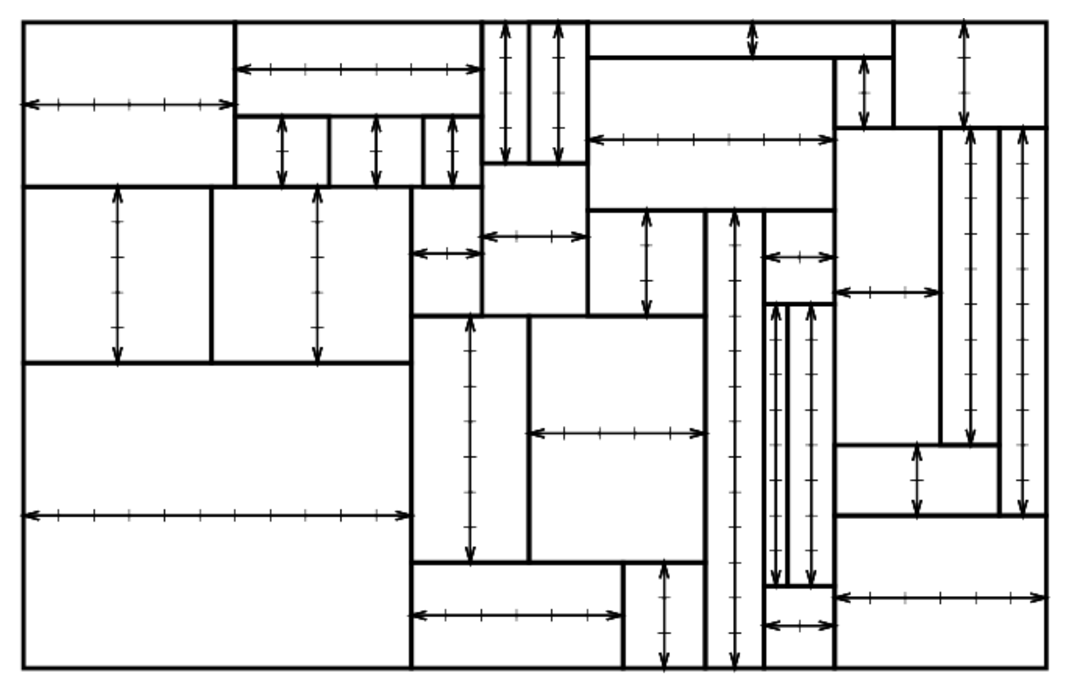
\includegraphics[scale=0.6]{Figs/Insight/rect}
\end{figure}

\subsection*{Весы и гири} %(TIPPING THE SCALES)

На столе у учителя стоят чашечные весы, правая чашка весов перевешивает.
На весах стоят гири не обязательно одного веса, на каждой из которых написаны фамилии одного \emph{или нескольких} учеников.
Ученик, входя в класс, переставляет на другую чашку весов каждую гирю, на которой написана его фамилия.
Докажите, что можно впустить в класс таких учеников, чтобы в результате перевесила левая чашка весов.

\subsection*{Часы на столе} %(WATCHERS ON THE TABLE)

На столе лежат пятьдесят точных ручных часов.
Докажите, что существует момент времени, когда сумма расстояний от центра стола до кончиков минутных стрелок больше, чем сумма расстояний от центра стола до центров часов.

\subsection*{Путь по шахматной доске} %(PATH ON CHESSBOARD)

Алиса начинает игру и ставит фишку в угол шахматной доски размером $n{\times}n$ клеток.
Боб передвигает фишку на соседнее поле, имеющее общую сторону с тем, на котором стоит фишка.
Второй раз ходить на поле, где уже побывала фишка, нельзя. 
Алиса и Боб ходят по очереди.
Проигрывает тот, кому некуда ходить.

При каких $n$ у Алисы есть выигрышная стратегия? 
При каких $n$ она выигрывает, если ее первый ход не на угловое поле, а на соседнее с ним?

\subsection*{Степень в степени} %(EXPONENT UPON EXPONENT)

На экзамене по математике для старших классов Американской школы 1960-х годов 
был следующий вопрос:
Если 
$$x^{x^{x^{{\cdot}^{\cdot^{\cdot}}}}}=2$$
Чему равен $x$? 
Предполагаемое решение основывается на том, что степень «нижнего» $x$ равна всему выражению, таким образом $x^2\z=2$ и $x=\sqrt{2}$.
Но один ученик заметил, что если бы в задаче спрашивалось решение
$$x^{x^{x^{{\cdot}^{\cdot^{\cdot}}}}}=4$$
то он бы получил тот же ответ: $x=\sqrt[4]{4}=\sqrt{2}$

Хмм...
Чему же тогда равно ${\sqrt{2}}^{{\sqrt{2}}^{{\sqrt{2}}^{{\cdot}^{\cdot^{\cdot}}}}}$? 
Можете это доказать?

\subsection*{Солдаты в поле} %(SOLDIERS IN THE FIELD)

Нечётное число солдат расположилось на поле таким образом, что все попарные расстояния между ними (между каждой парой солдат) различны.
При этом каждый солдат должен присматривать за ближайшим к нему другим солдатом.

Докажите, что существует хотя бы один солдат, за которым никто не присматривает.

\subsection*{Отрезки и расстояния} %(INTERVALS AND DISTANCES)

Пусть множество $S$ состоит из $k$ непересекающихся отрезков, лежащих в единичном отрезке $[0,1]$.
Предположим, что $S$ обладает следующим свойством: для любого вещественного числа $d$ из отрезка $[0,1]$, в множестве $S$ существуют две точки на расстоянии $d$ друг от друга.
Докажите, что сумма длин отрезков $S$ не меньше $1/k$.

 
\subsection*{Собрать 15} %(SUMMING TO 15)

Алиса и Боб по очереди выбирают число из $1, 2,\dots,9$, без повторов.
Выигрывает тот, кто первый наберет три числа, дающие в сумме 15.
Имеется ли у Алисы (она ходит первая)
выигрышная стратегия?

%ё
\section*{Решения и комментарии}

\subsubsection*{Два Биксби} % (THE BIXBY BOYS)

Классическая головоломка.
Конечно же, это были тройняшки.
Третий близнец (Арнольд?) учился в другом классе.

\subsubsection*{Свет на чердаке} % (THE ATTIC LAMP SWITCH)

Эта задача пронеслась по миру, как эпидемия гриппа, где-то лет десять тому назад; я не знаю её источника.

Действительно, невозможно определить, какой выключатель подключён к лампочке на чердаке, если всё, что у вас имеется --- это один бит информации, полученный от вашего похода на чердак.
Однако, вы можете добыть больше сведений, если используете ваши руки!
Включите выключатели 1 и 2, подождите несколько минут, затем выключите второй выключатель и идите на чердак.
Если лампочка не горит, но горячая, значит, второй выключатель это то, что мы ищем.
\heart

Если вы не можете дотянуться до лампочки, но обладаете огромным терпением, вы можете добиться того же результата, включив второй выключатель и подождав пару месяцев, затем включить первый выключатель и посетить чердак.
Если лампочка перегорела, то виноват в этом второй выключатель.

\subsubsection*{Бензиновый кризис} %(GASOLINE CRISIS)

Эта задача была известна довольно давно, вы можете найти её, например, в чудесной книге Ласло Ловаса\footnote{Laszlo Lovasz, \emph{Combinatorial Problems and Exercises}.}.
Трюк заключается в следующем:
представьте, что вы начинаете на автозаправке, скажем, №\,1 с достаточным количеством бензина и затем продолжаете свой путь, опустошая каждую автозаправку на кольцевой дороге.
Когда вы вернётесь к заправке №\,1, 
у вас будет столько же бензина, как и в начале пути.

Во время поездки записывайте, сколько бензина у вас остаётся перед каждой заправочной станцией.
Предположим, что это количество минимально перед автозаправкой №\,$k$.
Значит, если вы начнёте с автозаправки №\,$k$ с пустым баком, вы не рискуете оказаться без бензина на дороге между заправочными станциями.\heart

\subsubsection*{Бикфордовы шнуры} %(USES OF FUSES)

Подожгите одновременно оба конца первого шнура и один конец второго.
Когда первый шнур сгорит (через полминуты), подожгите незажжённый конец второго шнура.
К моменту, когда он догорит полностью, пройдёт 45 секунд.
\heart

Несколько лет назад эта и другие задачи о бикфордовых шнурах распространились по миру, как лесной пожар.
Дик Хесс, эксперт по занимательной математике, 
собрал небольшую книжку таких задач.\footnote{Dick Hess and Jerry Slocum, \emph{Shoelace Clock Puzzles}.}
Сам он впервые услышал приведённую выше задачу от Карла Морриса из Гарвардского университета.

Хесс рассматривает бикфордовые шнуры (он их зовёт шнурками) различной длины, но поджигает их только с концов.
Если же вам позволено поджигать шнур во внутренних точках и вы обладаете определённой ловкостью, то можно добиться гораздо большего.
Например, можно отмерить 10 секунд с помощью одного 60-секундного шнура, если зажечь его с обеих концов и в двух внутренних точках, а затем, каждый раз, когда сегмент сгорает, поджигать в новой внутренней точке.
Таким образом, у вас всё время горят три сегмента с двух концов, и шнур сгорает в шесть раз быстрее.

Будет немного суеты под конец и, конечно же, понадобится бесконечное число спичек, чтобы достичь абсолютной точности.

\subsubsection*{Целые числа и прямоугольники} %(INTEGERS AND RECTANGLES)}

Эта задача была предметом особой 
статьи Стэна Вэгона.%
\footnote{Stan Wagon “Fourteen proofs of a Result about Tiling a Rectangle”, American Mathematical Monthly Vol. 94, (1987) pp 601--617.}

Некоторые из решений, предложенных Вэгоном, забавным образом используют мощную математическую технику.
А одно решение не из их числа, предлагает нам следущее:
наложим на большой прямоугольник сетку, состоящую из квадратов со стороной 1/2, так, чтобы нижний левый угол прямоугольника находился в вершине клетки сетки.
Раскрасив клетки сетки в белый и чёрный цвета в шахматном порядке, 
мы видим, что каждый малый прямоугольник ровно наполовину белый и наполовину чёрный.
Следовательно, то же будет верно и для большого прямоугольника.
Но, допустим, высота большого прямоугольника не целое число, тогда часть 
большого прямоугольника между линиями $x=0$ и $x=1/2$ не содержит одинаковое количество белого и чёрного цвета.
Следовательно, основание должно быть целым числом.\heart

Автор книги несёт ответственность за следующее решение, которое вы не найдёте в статье Вэгона.
Пусть $\varepsilon$ меньше, чем наименьшая допустимая длина стороны прямоугольника разбиения.
Раскрасим каждый малый прямоугольник с целым основанием зелёным цветом, кроме красных горизонтальных полосок шириной $\varepsilon$ вдоль его верхней и нижней сторон.
Раскрасим оставшиеся прямоугольники красным, за исключением зелёных вертикальных полосок шириной $\varepsilon$ вдоль левой и правой сторон.

%в решении ссылаются на цвета диаграмы, но при печати она станет ч/б
\begin{figure}[h!]
\centering
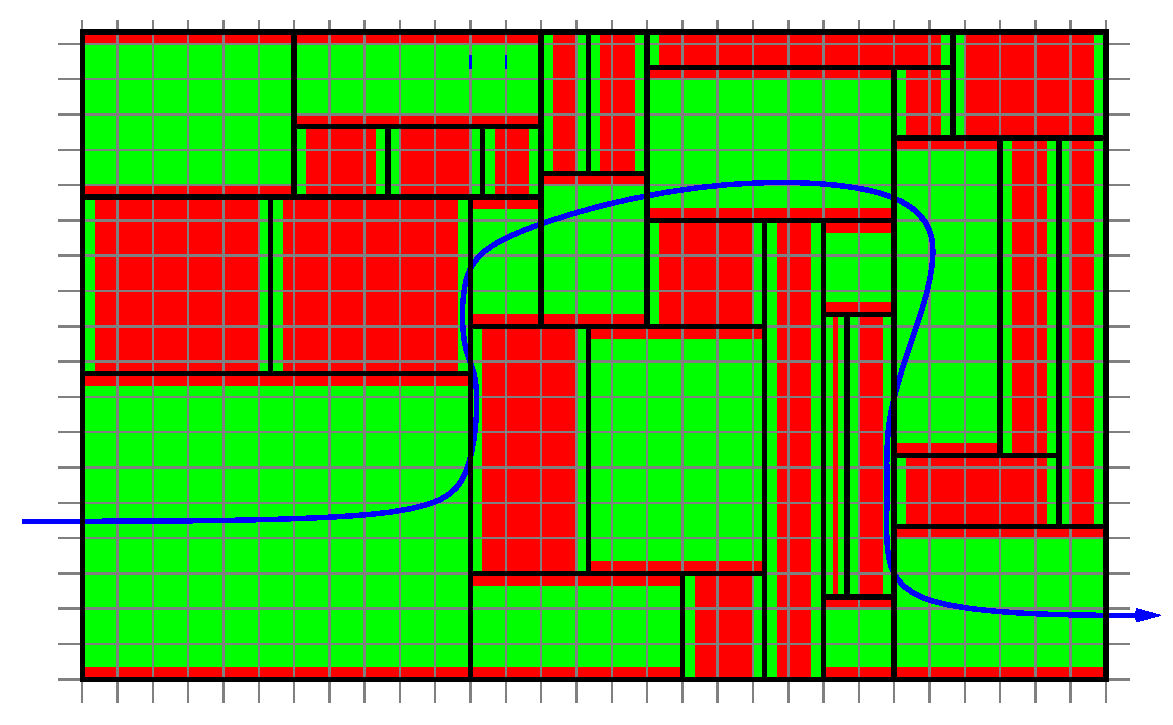
\includegraphics[scale=0.5]{Figs/Insight/green}
\end{figure}

Поместим в нижний левый угол большого прямоугольника начало координат.
Заметим, что у нас есть либо зелёный путь с левой стороны большого прямоугольника до его правой стороны, либо красный путь с нижней стороны до верхней.
Рассмотрим первый вариант.
Каждое место пересечения зелёного пути с вертикальными сторонами малых прямоугольников имеет целую координату; таким образом, основание большого прямоугольника --- целое число.
Подобным же образом и красный путь снизу вверх определяет целую высоту.

\subsubsection*{Весы и гири} %(TIPPING THE SCALES)

Рассмотрим результат для каждого подмножества учеников, включая пустое.
Заметьте, что каждая гиря окажется на левой чашке весов ровно в половине случаев.
В частности, средний вес гирь на левой чашке для всех подмножеств учеников равен их среднему весу на правой чашке.
Поскольку для пустого множества правая чашка тяжелее, 
для какого-то другого множества тяжелее должна быть левая.\heart

\noindent{\small Источник: Вторая Всесоюзная математическая олимпиада, Ленинград, 1968.}

Техника «усреднения», описанная выше, часто используется: будьте внимательны!

\subsubsection*{Часы на столе} %(WATCHERS ON THE TABLE)

Рассматривая только одни часы, 
мы видим, что в течении одного часа среднее расстояние от центра стола $C$ до кончика минутной стрелки $M$ превышает расстояние от $C$ до центра часов $W$.
Действительно, если провести через точку $C$ прямую $L$, перпендикулярную прямой $CW$, 
то среднее расстояние от прямой $L$ до точки $M$, очевидно, равно $LW$, 
что, в свою очередь, равно $CW$.
Но расстояние $CM$, по меньшей мере, равно $LM$, а обычно больше.

Взяв сумму по всем часам, приходим к аналогичному заключению, и отсюда следует, что есть момент в течении одного часа, когда желанное неравенство выполняется.\heart

\begin{figure}[h!]
\centering
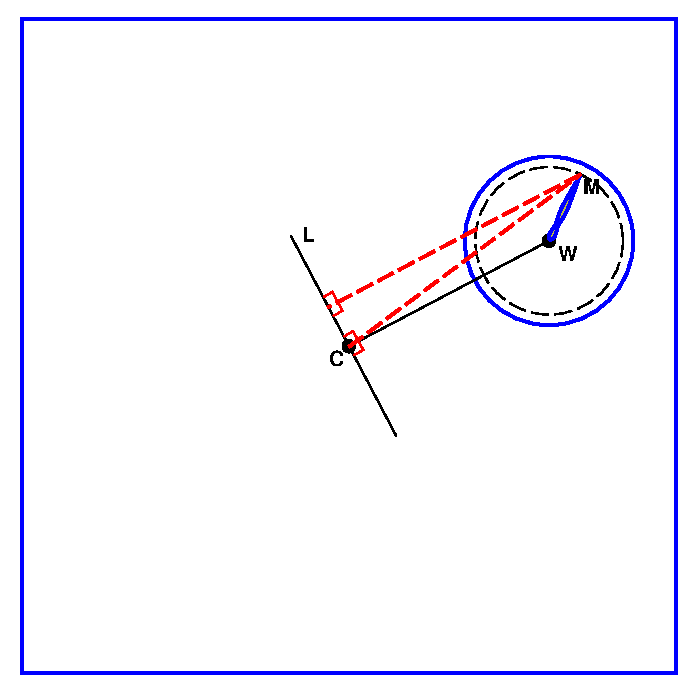
\includegraphics[scale=0.9]{Figs/Insight/watch}
\end{figure}

Требование точности часов обеспечивает движение каждой минутной стрелки с постоянной скоростью.
Это не так уж важно, когда скорости различаются, если только наше терпение не ограничено одним часом.

Одно дополнительное замечание: если установить и расположить часы определённым образом,
то \emph{можно} добиться того, что сумма расстояний от центра стола до кончиков минутных стрелок всегда была строго больше, чем сумма расстояний от центра стола до центров часов.\heart

\noindent{\smallИсточник: данная задача впервые появилась на десятой Всесоюзной математической олимпиаде в Душанбе, 1976.}

\subsubsection*{Путь по шахматной доске} %(PATH ON CHESSBOARD)

Если $n$ --- чётное число, у Боба имеется простая выигрышная стратегия, независимо от того, где Алиса начинает.
Он просто представляет себе, что шахматная доска покрыта прямоугольничками размером $1{\times2}$ клетки (домино) и каждый раз ставит фишку на вторую клетку того домино, куда пошла Алиса («закрывает» домино). %???обычно говорят «доминошки»
(Заметим, что эта стратегия работает для Боба, даже если Алисе разрешено ставить фишку на любую клетку при каждом ходе!).

Если $n$ --- нечётное, и Алиса начинает с угла, она выигрывает, если представит, что домино покрывает всю доску, кроме угловой клетки, с которой она начинает.

Tем не менее, Алиса проигрывает в случае с нечётным $n$, если она должна начинать с клетки, соседней к угловой.
Предположим, угловые клетки на данной доске чёрные, то есть Алиса начинает с белой клетки.
Существует покрытие всей шахматной доски домино, за исключением одной чёрной клетки.
Боб выигрывает, «закрывая» все домино.
Алиса
никогда не сможет поставить фишку на незакрытую клетку, потому что все клетки, на которые она ходит --- белые.\heart

\noindent{\small Источник: Двенадцатая Всесоюзная математическая олимпиада, Ташкент, 1978.}

\subsubsection*{Степень в степени} %(EXPONENT UPON EXPONENT)

Если выражение
$${\sqrt{2}}^{{\sqrt{2}}^{{\sqrt{2}}^{{\cdot}^{\cdot^{\cdot}}}}}$$
имеет какой-то смысл, то это не что иное, как предел последовательности
$${\sqrt{2}}, {\sqrt{2}}^{{\sqrt{2}}}, {\sqrt{2}}^{{\sqrt{2}}^{{\sqrt{2}}}},\dots$$
Этот предел существует, так как последовательность возрастает и ограничена.

Для доказательства первого утверждения, обозначим эту последовательность
$s_1, s_2,\dots$ и докажем по индукции, что $1<s_i\z<s_{i+1}$
для каждого $i\ge 1$.
Это сделать легко, поскольку \[s_{i+2}=
{\sqrt{2}}^{s_{i+1}}
>{\sqrt{2}}^{s_{i}}
=s_{i+1}.\]

Для нахождения верхней грани, заменим самую верхнюю степень в каждом $s_i$ на б\'{о}льшее число $2$, тогда всё выражение превращается в двойку.

Теперь, когда мы знаем, что предел существует, обозначим его $y$.
Он должен удовлетворять уравнению ${\sqrt{2}}^y=y$.
Рассмотрев уравнение $x=y^{1/y}$, 
можно увидеть, применив элементарный матанализ (приношу извинения!), 
что $x$ строго возрастает при возрастании $y$ до максимума при $y=e$
и после чего убывает.
Таким образом, существует не больше двух значений $y$, для данного $x$, 
и при $x=\sqrt{2}$ нам известны оба: $y=2$ и $y=4$.

Поскольку наша последовательность ограничена сверху двойкой, можно исключить $4$ и, таким образом, $y=2$.\heart

Обобщив приведённое выше доказательство, мы видим, что выражение $x^{x^{x^{{\cdot}^{\cdot}}}}$
имеет смысл и равно наименьшему решению уравнения $x=y^{1/y}$ при $x\le e^{1/e}$.
При $x=e^{1/e}$, выражение равно $e$ но как только $x$ превысит $e^{1/e}$, последовательность устремляется к бесконечности.

\subsubsection*{Солдаты в поле}%(SOLDIERS IN THE FIELD)

Данная задача была представлена на шестой Всероссийской математической олимпиаде в Воронеже, 1966.
Её легче всего решать, начав с двух солдат, находящихся друг от друга на кратчайшем расстоянии.
Ясно, что они присматривают друг другом, и если кто-то ещё смотрит на одного из них, тогда у нас имеется солдат, за которым присматривают дважды и, значит, есть солдат, за которым никто не присматривает.
Если же за этими двумя солдатами больше никто не присматривает, то можно их убрать, не влияя на остальных.

Так как число солдат нечётное, то, применяя и далее это рассуждение, мы, в конце концов, придём к одному солдату, который ни за кем не присматривает --- противоречие.\heart

\subsubsection*{Отрезки и расстояния} %(INTERVALS AND DISTANCES)

{\small Источник: Семнадцатая Всесоюзная математическая олимпиада, Кишинёв, 1983.}

Обозначим через $s_1,\dots,s_k$ длины отрезков множества $S$,
пусть их сумма равна $s$.
Рассмотрим интервал $I_{ij}$, содержащий все расстояния, которые можно получить, взяв первую точку на $i$-том и вторую на $j$-том отрезке множества $S$.
Ясно, что длина $I_{ij}$ равна $s_i+s_j$.
Суммируя по всем парам $i\ne j$, 
каждая длина появляется $k-1$ раз,
таким образом, сумма длин интервалов по всем парам различных отрезков, не превосходит $(k-1) s$.
Расстояния между точками, взятыми из $i$-ого отрезка, имеют значения от $0$ до $s_i$.
Значит, общая длина всех интервалов $I_{ij}$ не превосходит $k s$.
Поскольку $k s\ge 1$, получаем $s\ge 1/k$.
\heart

Равенство достигается, если максимум всех $s_i$ равен $s$, 
то есть если все отрезки, кроме одного, имеют нулевую длину.
Этого можно добиться взяв отрезок $[0,\tfrac1k]$ и добавив изолированные точки
$\tfrac2k,\tfrac3k,\dots,1$.

%исправлена фактическая ошибка --- отрезок можно брать только с краю, в середине брать нельзя.

\subsubsection*{Собрать 15} %(SUMMING TO 15)

Быстрый способ решить данную задачу --- это представить, что Алиса и Боб пользуются следующим магическим квадратом:
$$
\begin{matrix}
8&1&6\\
3&5&7\\
4&9&2
\end{matrix}
$$
Так как числа в строчке, столбике и диагонали дают в сумме 15, то можно сказать, что они играют в крестики-нолики! 
Всем известно, что наилучшая игра в крестики-нолики приводит к ничьей,
то есть ответ на наш вопрос --- нет, у Алисы нет выигрышной стратегии.
\heart

Эта забавная игра упоминается во втором томе классической книги Элвина Берлекампа, Джона Конвея и Ричарда Гая.\footnote{Winning Ways for Your Mathematical Plays by Elwyn Berlekamp, John Conway and Richard Guy ; Academic Press, 1982: 2nd Edition, A K Peters 2001}
В книге задача приписывается некоему «Э. Периколозо Спорджерси»\footnote{E. Pericoloso Sporgersi}, что выглядит очень подозрительно --- такую надпись можно увидеть в итальянских поездах, она предупреждает пассажиров об опасности высовываться из окна.

\chapter*{География(!)}
\addcontentsline{toc}{chapter}{География(!)}

\setlength{\epigraphwidth}{.45\textwidth}
\epigraph{Без географии мы были бы нигде.}{---Джимми Баффет (1946---)}%???- или --- 

Да, данная глава не принадлежит этой книге. %(не из этой книги).
Некоторые из задач, представленных здесь, конечно, математические по своей природе, %(mathematical in nature) 
но, в основном, они включены в книгу потому, что доставляют, как мне кажется, большое удовольствие любителям математических головоломок.
Мой издатель уверял меня, что без «Географии» стоимость книги была бы такой же.

Так что эта глава как бы бесплатное приложение, и её можно пропустить с чистой совестью.

Основная тема приведённых ниже задач --- поверхность планеты Земля.
Хотя предпочтение всё-таки отдаётся моей родине --- Соединённым Штатам Америки. 
О чём прошу прощения у читателей из других стран.
Я буду очень благодарен за подобные задачи про разные страны, присланные мне на pw@akpeters.com.

Несколько из этих задач показывают до какой степени %( test the degree) 
картографическая проекция %( на плоскость) (planar projections) 
искажает наше представление о земном шаре. %(глобусе, globe).
Вот одна из них: 

\subsection*{Африка}
\rindex{Африка}

Какой штат США ближе всего к Африке? 

\paragraph{Решение:} Штат Мэн.\heart
  
Он совсем не близко --- проверьте по глобусу.
Но если вы летите по ортодромии (в картографии и навигации ортодромия --- название кратчайшего расстояния между двумя точками на поверхности Земли) из Майами, скажем, в Касабланку, вначале ваш курс %(путь)
будет лежать на Северо-Восток вдоль восточного побережья и пройдёт очень близко к штату Мэн.
%(not missing Maine by much)

\medskip

Дальше попробуйте сами.

\subsection*{На восток от Рино}%EAST OF RENO 
\rindex{На восток от Рино}

Какой самый большой город в США к востоку от Рино, Невада и к западу от Денвера, Колорадо? 

\subsection*{Телефонный звонок}%(THE PHONE CALL) 
\rindex{Телефонный звонок}

Представьте, что вы звоните из какого-то штата Восточного побережья в один из штатов Западного побережья США, и на обеих концах одно и то же время суток.
Как такое может быть? 
  

\subsection*{Диаметр Соединённых штатов}%(THE DIAMETR OF US)  
\rindex{Диаметр Соединённых штатов}

В каких двух штатах находятся две самые удалённые точки США? 
  

\subsection*{На юг от Ки-Уэст}% ( SOUTH FROM KEY-WEST) 
\rindex{На юг от Ки-Уэст}

Если вы летите на юг от города Ки-Уэст, Флорида, какая южно-американская страна вам 
встретится первой? 

\subsection*{Индейцы на среднем западе}% (INDIANS IN THE MIDWEST) 
\rindex{Индейцы на среднем западе}

Среди штатов Среднего Запада США только один имеет название не индейского происхождения? Который?    

\subsection*{Самый большой второй по величине город}% (THE LARGEST SECOND-LARGEST CITY)  
\rindex{Самый большой второй по величине город}

Какой город в США самый большой среди городов с одинаковыми именами, но не больше города США с таким же именем?

\medskip

Эта формулировка может показаться несколько путаной.
Спросим по-другому: скажем, что город (в США) «находится в тени», если существует б\'{о}льший город с таким же именем.
Например, Портланд, штат Мэн, находится в тени города Портланд, штат Орегон.

Итак, наш вопрос прозвучит теперь так: какой наибольший город в США находится в тени?   

\subsection*{Естественные границы}% (THE NATURAL BORDERS) 
\rindex{Естественные границы}

Граница штата может быть естественной (определяться водоёмами, горами и пр.) или 
закреплённой в законе искусственной линией --- в одном знаменитом случае (связанном со штатом Делавэр и Пенсильванией ) --- это дуга окружности.
Три штата --- Колорадо, Юта и Вайоминг имеют только искусственные границы.
Какой штат обладает только естественными границами?   

\subsection*{Непересекаемые границы}% (THE UNCROSSABLE BORDER) 
\rindex{Непересекаемые границы}

Говоря о границах штатов, можете ли вы найти такой штат, который нельзя пересечь на автомобиле? Другими словами укажите два штата, имеющих общую границу, через которую, однако, невозможно напрямую проехать на автомобиле из одного штата в другой?   

\subsection*{Отдел странных названий}% (DEPARTMENT OF ODD NAMES) 
\rindex{Отдел странных названий}

Что особенного в неком местечке, именуемом Уэст-Куодди-Хед, %(West Quoddy Head) 
штат Мэн?   

\subsection*{Городской и деревенский}%(URBAN AND RURAL) 
\rindex{Городской и деревенский}

Данная задача скорее более социологического плана.
В наши дни большинство американцев --- порядка 75\% --- живут в так называемых «городских агломерациях (урбанизированных зонах)».
Перепись населения 2000 года относит к «городскому» 100\% населения одного из штатов и только 27,6\% населения другого штата, который отдалён от первого всего лишь на несколько сот миль.
Можете назвать эти два штата?   

\subsection*{Города на север и на юг}% (CITIES NORTH AND SOUTH) 
\rindex{Города на север и на юг}

Как обстоит дело с вашей визуализацией континентов?
Проверьте, как точно вы представляете себе %(визуаилизируете) 
карту мира.
Расставьте следующие четыре города по порядку с юга на север: 
Галифакс, Новая Шотландия; %(Halifax, Nova Scotia) 
Токио, Япония; %(Tokyo, Japan); 
Венеция, Италия; %(Venice, Italy); 
Алжир, Алжир. %(Algiers, Algeria).

\subsection*{Город в один слог}% (THE ONE-SYLLABLE CITY) 
\rindex{Город в один слог}

Какой город в США, имя которого состоит из одного слога, самый большой? 

\subsection*{Вашингтоны и феминисты}%(WASHINGTONS AND FEMINISTS) 
\rindex{Вашингтоны и феминисты}

Данная задача --- это своеобразный тест на знание не только карты штатов США, но и их английских названий.
Чтобы найти решение этой задачи, вам придётся пользоваться исключительно оригинальными английскими названиями штатов.
Итак, вопрос: 

Сможете ли вы проложить маршрут для автомобиля из города Сиэтл, штат Вашингтон, 
 в Вашингтон, округ Колумбия, таким образом, чтобы названия всех штатов, через которые вы планируете проехать, начинались только с букв, составляющих слово «WOMAN»?
%???добавленно 

\medskip

Наша последняя географическая задача напоминает нам, что пора возвращаться к математике. %(signals us a(slight) return to mathematics) направляет 

\subsection*{Учёный и медведь}%(THE NATURALIST AND THE BEAR) 
\rindex{Учёный и медведь}

Учёная-биолог покинула лагерь экспедиции, прошла 10 миль на юг, затем 10 миль на восток и тут заметила и сфотографировала медведя.
Пройдя 10 миль на север, она пришла обратно в лагерь.

\medskip

Вы не видели фотографии, но всё равно знаете, какого цвета был медведь, не так ли?

\section*{Решения и комментарии}


Для проверки правильности ответов  бы можете воспользоваться атласом, глобусом, альманахом  или итогами переписи населения США 2000 года. 
Давайте посмотрим, насколько верны были ваши предположения...
%(догадки)


\subsubsection*{На восток от Рино}% (EAST OF RENO)


Вопрос о самом большом городе может оказаться довольно щекотливым; 
%(awkward question)  
стандартно  это понятие определяется количеством  населения (не площадью!) в официальных границах города, что, безусловно, может привести к неверным выводам
при наличии  городских агломераций (урбанизированных зон).
%(can be misleading with respect to metropolitan area).
Так, например, согласно данным альманаха город Джэксонвилл, штат Флорида, представляется больше, чем Атланта, штат Джорджия,  несмотря на то, что население всей городской агломерации Атланты превышает население Джэксонвилла почти в четыре раза.


Но в нашей задаче нам не понадобятся такие тонкости. Самый большой город к востоку от Рино  и к западу от Денвера, в любом случае, Лос-Анджелес, Калифорния.                                                                                                                                  \heart






\subsubsection*{Телефонный звонок}%ТЕЛЕФОННЫЙ ЗВОНОК (THE PHONE CALL)


«Восточное побережье»  Соединённых Штатов Америки включает в себя  восточные штаты, имеющие выход к Атлантическому океану,  от штата Мэн на севере до штата Флорида на юге. 
К «Западному  побережью»  относятся штаты Вашингтон, Орегон и Калифорния,
к  которым, если хотите, вы можете добавить Аляску и даже Гавайи,  но это не так уж важно в данном случае. %(but it doesn’t help).


Обычно, делая подобные звонки, мы имеем разницу во времени между Восточным и Западным побережьем в 3 часа.  Мы можем избавиться от одного часа, позвонив из  западного района так называемой  «ручки ковша» Флориды --- её северо-западной части, % ( Florida panhandle) 
скажем, из города Пенс\'акола, который находится в  Центральном часовом поясе.  
Чтобы избавиться ещё от одного часа, мы звоним в один из городов самого  восточного района  штата Орегон (скажем, Онтарио),  в котором Горное время. 
Оставшийся час исчезнет, если звонок будет сделан  из Пенс\'аколы между двумя и тремя часами ночи, при переходе с Летнего времени на Зимнее. 
В этот момент в Центральном часовом поясе время уже переведут на один  час назад, а Горное время все ещё  будет прежним.\heart   


                            
                                                                                                                                     
\subsubsection*{Диаметр Соединённых штатов}%ДИАМЕТР СОЕДИНЁННЫХ ШТАТОВ (THE DIAMETR OF US) 


Очевидно, это либо Гавайи и Мэн, либо Аляска и Флорида. Или это Гавайи и Аляска?


Удивительным образом, ни одно, ни другое, ни третье.  Правильный ответ --- Гавайи и Флорида.\heart




\subsubsection*{На юг от Ки-Уэст}%НА ЮГ ОТ КИ-УЭСТ ( SOUTH FROM KEY-WEST)


Это, без сомнения, каверзный  вопрос. %(a trick question).  
Вы не пересечёте ни одну страну Южной Америки. 
Ваш путь пройдет к западу от континента. 
(Ваш путь пройдет вдоль западного побережья всего континента.)\heart


\subsubsection*{Индейцы на среднем западе}%ИНДЕЙЦЫ НА СРЕДНЕМ ЗАПАДЕ (INDIANS IN THE MIDWEST)


По определению к штатам  Среднего Запада относятся Миннесота, Висконсин, Айова,
Иллинойс, Миссури, Мичиган, Огайо, Канзас и Небраска --- все названия индейского
происхождения, и остается ответ --- Индиана!\heart


Любопытно, что только один штат к востоку от Миссисипи имеет столицу, чье имя индейского происхождения --- Флорида (Таллахасси).




\subsubsection*{Самый большой второй по ввеличине город}%САМЫЙ БОЛЬШОЙ ВТОРОЙ ПО ВЕЛИЧИНЕ ГОРОД (THE LARGEST SECOND-LARGEST CITY)     


Портланд, штат Мэн, Спрингфилд, что-то?  Популярные предположения, но не верные.
До 1975 года или около того, правильный ответ был бы Канзас-Сити, штат Канзас, который затеняется городом Канзас-Сити, Миссури.
Затем некоторое время победителем был Колумбус, Джорджия, находящийся в тени столицы Огайо. Однако, мы живем в эпоху пригородов, %(in the age of suburbia), 
перепись населения 2000 года показывает, что теперь городу Глендейл, штат Калифорния (находится в тени Глендейла, Аризона) принадлежит эта сомнительная %(obscure) 
честь.\heart




\subsubsection*{Естественные границы}%ЕСТЕСТВЕННЫЕ ГРАНИЦЫ (THE NATURAL BORDERS)


Конечно, Гавайи  имеют только естественные границы. Возможно, вы подумали, что это было слишком легко, но люди часто не видят, что находится у них под носом. 
%(не замечают очевидного)  %(folks often have a blind spot).
\heart




\subsubsection*{Непересекаемые границы}%НЕПЕРЕСЕКАЕМЫЕ ГРАНИЦЫ  (THE UNCROSSABLE BORDER)


Здесь намного сложнее. Висконсин и Мичиган имеют общую длинную границу по озеру Мичиган, но вы можете пересечь её на пароме Манитовок-Ладингтон, сидя в своей машине. Паром из Монток Пойнт %(Mantauk Point) 
(штат Нью-Йорк) на остров Блок %(Block Island) 
(штат Род-Айленд) пересекает не очень хорошо известную границу между этими двумя штатами, и он только для пассажиров. 
Возможно, существуют и другие решения данной задачи.\heart
                                                                                                                    


Можно задать схожий вопрос о части штата, попасть в которую на автомобиле из остального штата возможно только, проехав через другой штат (или Канаду, в случае с 
Пойнт Робертс. %(Point Roberts). 
Существует несколько таких мест, особенно около вечно изменчивой реки Миссисипи.




\subsubsection*{Отдел странных названий}%ОТДЕЛ СТРАННЫХ НАЗВАНИЙ (DEPARTMENT OF ODD NAMES)


Уэст-Куодди-Хед %(West Quoddy Head) 
--- самая восточная точка континентальных штатов США.\heart
                                                                                                                


Иногда вам может встретиться утверждение,  что, если опустить  требование «континентальный», мыс Врангеля %(Cape Wrangel) 
на острове Атту, %(Attu Island) 
штат Аляска, является самой восточной точкой США,  но я не принимаю в рассчет эти «Гринвич-централизованные»  доводы. 
%(but I do not buy Greenwich-centered reasoning) 
Назовёте ли вы мыс Врангеля самой восточной точкой Аляски?




\subsubsection*{Городской и деревенский}%ГОРОДСКОЙ И ДЕРЕВЕНСКИЙ (URBAN AND RURAL)


Нью-Джерси и Вермонт. Эту и множество другой интересной информации вы можете найти на сайте:\\
\texttt{http//www.census.gov/prod/2002pubs/01statab/pop.pdf} 
 \heart                                                                                                      




\subsubsection*{Города на север и на юг}%ГОРОДА НА СЕВЕР И НА ЮГ (CITIES NORTH AND SOUTH)


Токио, Алжир, Галифакс и, наконец, Венеция. Широты, соответственно
$35^\circ 40’$ с.ш.;  $36^\circ 50’$ с.ш.; $44^\circ 53’$ с.ш.; и $45^\circ 26’$ с.ш. 
Обратите внимание --- последние два города разделяет 45-я параллель, и это позволяет нам яснее увидеть, что Венеция находится севернее. Один уроженец Новой Шотландии однажды проспорил мне по этому случаю 1 доллар.\heart




\subsubsection*{Город в один слог}%ГОРОД В ОДИН СЛОГ (THE ONE-SYLLABLE CITY)


Йорк, штат Пенсильвания, и Трой, штат Нью-Йорк, называются чаще всего, но все же Флинт, штат Мичиган, несмотря на существенное сокращение населения за последние годы, остаётся единственным однослоговым городом в США с населением более 100 тыс. человек.  Хотя, если судить по тому, как произносят названия городов местные жители, победителем, несомненно, будет Нью-Арк («Норк», с длинным «о»),  штат Нью-Джерси. \heart






\subsubsection*{Вашингтоны и феминисты}%ВАШИНГТОНЫ И ФЕМИНИСТЫ (WASHINGTONS AND FEMINISTS)


Без проблем. Вначале ваш маршрут пойдет на юг ---  через Орегон (Oregon), 
Неваду (Nevada) 
и Аризону, (Arizona),  
затем на восток сквозь Нью-Мексико (New Mexico) 
в  Оклахомовскую «ручку ковша»,  из северо-восточного  угла Оклахомы (Oklahoma) 
вы попадаете в  Миссури (Missouri). 
Здесь вам надо будет повернуть на север и из северо-западного угла штата проехать в Небраску (Nebraska),  продолжая путь на  запад в Вайоминг (Wyoming)  и на север в Монтану (Montana) --- довольно большой круг для того, чтобы объехать Айдахо (Idaho). 
В конце концов, вы сможете снова развернуться и поехать на восток через Северную Дакоту (North Dakota), 
Миннесоту (Minnesota), 
Висконсин (Wiskonsin) 
и Мичиган (Michigan).
Теперь берите курс на юг в Огайо (Ohio) и на восток сквозь Западную Виргинию (West Virginia) в Мериленд (Maryland),
 и в Вашингтон (Washington DC), округ Колумбия.\heart


Чтобы пройти по этому маршруту, вам придется несколько раз (или на долгое время) покинуть национальную систему межштатных автомагистралей, но мы предполагаем,  вы никуда не торопитесь.


\subsubsection*{Учёный и медведь}%УЧЕНЫЙ И МЕДВЕДЬ  (THE NATURALIST AND THE BEAR)




Начальная идея была, конечно, что лагерь экспедиции находился на Северном полюсе, так как маршрут ученой (10 миль на юг, 10 миль на восток и 10 миль на север)  является замкнутым контуром, %(to have been a closed loop),  
следовательно  медведь был белый.


Однако, как было замечено в одной из рубрик %(колонок) 
Мартина Гарднера, %(Martin Gardner’s columns), 
на поверхности Земли существует бесконечно много других точек, где подобный путь будет замкнутым.


Некоторые из этих точек лежат на окружности  с центром в Южном полюсе и радиусом немного меньше $10 + 5/\pi$ миль.
Начав   прогулку с такой точки,  наша учёная после первых 10 миль окажется в некой точке $P$,  
находящейся на расстоянии чуть меньше $5/\pi$ миль от Южного полюса.  
Повернув на Восток и пройдя 10 миль, она обогнёт весь мир и вернётся в точку $P$, откуда 10 миль на Север приведут её обратно в лагерь.
Другая окружность, радиусом чуть меньше $10 +  5/\pi$ миль тоже сработает, во второй (Восточной) части пути наша учёная должна будет 2 раза обойти вокруг Южного полюса  и так далее.
В Антарктике медведи не водятся, но если бы водились, то, наверное, были бы белыми.
Так что ответ задачи не изменится.\heart
\end{document}
%ссылки  на источник даются в разном формате, я бы его униформуизировал 
%проверь разбивку на абзацы, иногда она у тебя не та, что у винклера 